\documentclass[conference]{IEEEtran}
\usepackage{amsmath,amssymb,amsthm}
\usepackage{graphicx}
\usepackage{booktabs}
\usepackage{array}
\usepackage{cite}
\usepackage[hidelinks]{hyperref}
\hypersetup{pdftitle={When Does More Detail Help a Regional Energy Twin?},pdfauthor={Alexander V. Mantzaris},pdfsubject={DSpaCES 2026 author-review case-study manuscript}}
\newtheorem{proposition}{Proposition}
\newcommand{\R}{\mathbb{R}}
\newcommand{\MarginChecks}{4608}
\newcommand{\MarginCertified}{4608}
\newcommand{\FineGainPercent}{18.3}

\title{When Does More Detail Help a Regional Energy Twin?}
\author{\IEEEauthorblockN{Alexander V. Mantzaris}
\IEEEauthorblockA{School of Data, Mathematical and Statistical Sciences\\
University of Central Florida\\
alexander.mantzaris@ucf.edu}}
\begin{document}
\maketitle

\begin{abstract}
Regional digital twins can expose finer state, acquire more measurements, or change which measurements they request. These operations have different consequences, even when all are called refinement. We examine them in a retrospective energy twin built from 167.93 million London smart-meter rows, with 4,194 eligible households and 52.11 million training readings. A fixed hierarchical Gaussian model supports regional, group and household queries on a GPU. Same-evidence refinement preserves registered posterior queries, but its retained-state reduction from 61.12 to 21.60 MB offers no advantage over streamed fine inference retaining 21.60 MB. In 112 replay episodes on eight development backgrounds, synthetic local disturbances expose aggregate blind spots. Additional fine observations reduce local one-hour mean absolute error from 0.1696 kWh for the tested adaptive policy to 0.1386 kWh for streamed fine inference. However, none of 96 demand disturbances changes the adaptive acquisition schedule. Reconstructed traces locate the failure between changed scores and unchanged actions. A rank-responsive correction changes three of 12 fresh disturbance schedules on four reused backgrounds, yet it, the original policy and random acquisition each localize only two events. New requests for affected meters arrive after the scored detection window. The study establishes a reproducible separation of representation, information and acquisition effects, rather than an adaptive-method advantage. Results remain exploratory, with synthetic disturbances and incomplete uncertainty calibration.
\end{abstract}
\begin{IEEEkeywords}
regional digital twins, data spaces, selective observation, Gaussian inference, smart-meter data
\end{IEEEkeywords}

\section{Introduction}
A regional energy twin may need to summarize demand across thousands of households while retaining the ability to inspect a changing local pattern. A stable regional total can conceal offsetting household changes. Conversely, exposing thousands of local state variables need not improve a forecast if the estimator receives no new evidence. The practical question is when the cost of additional detail produces information that changes a useful decision.

We investigate three questions. \textbf{RQ1:} under the same statistical model and evidence, what does changing representation preserve, and what resources does it change? \textbf{RQ2:} when aggregation hides local disturbances, what prediction or detection value do additional fine observations provide? \textbf{RQ3:} does a tested acquisition policy convert available shock information into useful decisions at a fixed observation budget?

Our platform is a retrospective, data-driven twin of a sampled Greater London household population. It uses real half-hourly meter observations from Low Carbon London~\cite{london}. Providers are simulated partitions of actual households. The consumer receives group summaries and can request selected household readings. The exchange interface therefore determines which evidence is available to inference and monitoring. This is a concrete data-space role, although the replay is neither a live federation nor an evaluation of organizational interoperability.

We use a fixed hierarchical Gaussian model to separate operations that are otherwise easily conflated. Representation refinement exposes a conditional distribution without changing the observations. Evidence acquisition adds legally available readings and can change regional as well as local predictions. Model enrichment changes the distribution itself. Only the first two operations are compared after the model is frozen. A GPU implementation supports structured inference, while acquisition traces record physical meter identities, times, requested values and budget decisions.

The findings are predominantly limiting. Exact query preservation survives changes to retained detail, but the memory saving disappears against a competent streamed fine comparator. Fine observations improve local forecasting on perturbed real backgrounds, yet the tested event policy does not change its schedule in response to any of the initial 96 demand disturbances. A targeted diagnostic shows that information often reaches its score without crossing its acquisition gate. A single correction changes some schedules but does not establish an advantage over simple acquisition.

The case-study contribution is threefold. First, matched-model and matched-evidence comparisons distinguish query preservation from prediction improvement and retained-state savings from capacity gains. Second, controlled disturbances characterize aggregate visibility against the actual observation interface, including within-group cancellation. Third, an observation-to-action audit links exposure, innovations, scores, decisions and outcomes, identifying why apparent policy responsiveness fails to improve the measured result. Standard Gaussian identities and observability arguments explain these findings; they are not presented as new inference theorems. The code, frozen configurations, traces and paper-generation scripts are available together~\cite{artifact}.

\section{Related Work and Scope}
Multiresolution inference already provides principled ways to represent local and global uncertainty. Katzfuss's multiresolution approximation uses a hierarchical basis construction for massive spatial data~\cite{katzfuss2017}. The multiresolution filter extends structured probabilistic inference through time, with an approximation of forecast covariance and exactness in identified special cases~\cite{mrf}. Hierarchical sparse Cholesky methods obtain scalable filtering from specified conditional structure~\cite{vecchia}. These methods do not justify arbitrary update locality merely because a model has groups. Our smaller fixed model admits exact conditional calculations, but it does not supersede their spatial models or scale guarantees.

Distributed low-rank inference communicates local sufficient quantities and recovers the centralized posterior under its model~\cite{distributed}. This is the closest mathematical baseline for our common-state and private-detail decomposition. Incremental inference is also established: iSAM2 edits affected parts of a Bayes tree and reuses conditional information~\cite{isam}. Locality depends on separator size, ordering and coupling. Our comparisons grant conventional message reuse and streamed prediction. We do not compare refinement only against rebuilding a dense global inverse.

Forecast reconciliation makes predictions coherent with aggregation constraints. MinT minimizes the trace of reconciled forecast-error covariance under its stated assumptions~\cite{mint}. We instead obtain regional and local queries from one joint model. This guarantees algebraic agreement within that model, not accurate household demand or calibrated intervals. The distinction is consequential when detailed conditional predictions remain available from a coarse representation.

Event-triggered estimation distinguishes measurements from information carried by transmission decisions. Sun and Work study normalized-innovation triggering with synthetic measurements representing nontransmission~\cite{sun}. Han et al. construct stochastic triggers that preserve a Gaussian estimation structure under particular assumptions~\cite{han}. Our heuristic acquisition rule does not inherit those guarantees. It receives scheduled probes and ignores selection information from history outside its finite inference window.

Controlled sensing jointly chooses observations and a stopping rule. Veeravalli et al. establish first-order asymptotic optimality for a windowed procedure under finite action and post-change parameter sets, specified observation laws and a mean-time-to-false-alarm criterion~\cite{controlled}. Our fixed reading budget, empirical thresholds and perturbed meter backgrounds do not satisfy that setup. Random acquisition is an implemented simple comparator, not a claim to cover optimal active sensing.

Electricity anomaly detection may already use fine inputs before making an aggregate decision. He et al. use participant-level time-slot features and a participant localization rule~\cite{he}. Their interface is not an aggregate-only consumer with a small observation budget. We therefore compare information access explicitly rather than identifying a low-dimensional model with a coarse observation interface. The unresolved contribution is empirical: what the separated comparisons and causal execution traces reveal in this regional prototype. We make no claim that residual triggering, sufficient-statistic exchange or synthetic anomalies are novel.

\section{Regional Twin and Information Interfaces}
\subsection{Physical observations and study population}
Each reading is electricity consumed during a half-hour interval, measured in kWh. A one-hour forecast predicts the reading two intervals ahead; it is not an integral over the next hour. Six-hour forecasts similarly target the reading 12 intervals ahead. We retain meter identifiers and source clock labels. There are no verified feeders, borough assignments, coordinates or population expansion weights.

The source archive contains 167,932,474 rows, 167,817,021 distinct meter/time keys and 5,566 distinct meter identifiers. These locally counted figures differ from the catalog's approximate 167 million readings and 5,567 households~\cite{london}. One 801.67 MB ZIP expands to 8.54 GB of CSV and becomes 528.82 MB of typed, partitioned Parquet. Streaming ingestion processes about 472,000 rows/s, with 3.36 GB peak host memory. These are ingestion measurements, not inference throughput.

Nonfinite, invalid and negative readings become missing values. Duplicate keys are retained deterministically for archival bookkeeping but excluded from fitting and replay. Missing demand is never zero-filled as an outcome. Because the source does not resolve timezone and daylight-saving semantics sufficiently for this study, accessible clock-transition days are excluded. We do not invent UTC alignment.

Eligibility is fixed using 2012 only, requiring at least 8,760 valid training readings per household. The resulting 4,194-household cohort contributes 52,109,356 valid training readings. About 29.3\% of its rectangular training grid is missing. Of these households, 3,362 have standard and 832 time-of-use tariff labels. Tariff membership is recorded descriptively; this study does not estimate a tariff effect. January--March 2013 supplies exploratory development replay. April--December 2013 remains sealed, as do outcomes from an earlier, separate building-data project. Ingestion partitions held-out records but fitting, selection and scoring do not use their values.

\subsection{One fixed probabilistic model}
Let $y_{it}$ be household $i$'s recorded demand. The model is
\begin{align}
 s_{t+1}&=F_s s_t+\eta_t,\\
 y_{it}&=\mu_{i,\ell(t)}+\ell_i^\top s_t+d_{it}+\epsilon_{it},\label{eq:model}\\
 d_{i,t+1}&=\rho_i d_{it}+\zeta_{it}.
\end{align}
Here $s_t\in\R^{16}$ captures common variation, $\mu_{i,\ell(t)}$ is a 336-slot weekly seasonal profile, and $d_{it}$ is a private household residual. Loadings, dynamics and noise conventions are fitted on training data. Missing standardized residuals are mean-filled for initial factor construction only; loadings are refitted on observed entries. Private residual covariance uses a fixed 80\% autoregressive and 20\% nugget split, with persistence clipped to $[-0.95,0.95]$. The common transition has spectral radius 0.9942. These are working Gaussian assumptions, not verified physical laws.

Private innovations are conditionally independent given the common state. Household forecast errors are not unconditionally independent. The regional variance includes common-state uncertainty, future common process noise, private temporal dependence and measurement noise. Gaussian predictions may assign mass to negative demand; the inference model does not enforce a physical nonnegativity constraint. Disturbance generation does enforce nonnegative replay observations and targets.

Sixteen groups are formed by sorted physical meter index modulo 16. They contain 262 or 263 households and are synthetic consumption populations, not geographical neighborhoods. The finite window has 24 half-hour steps. Stacking common coordinates gives a separator of dimension $16\times24=384$. Including all private trajectories yields 101,040 formal coordinates at the largest cohort, but the implementation never forms a dense covariance of that size. Many source records contribute to fitted statistics; they are not all simultaneously resident in the GPU working set.

\begin{figure*}[!t]
\centering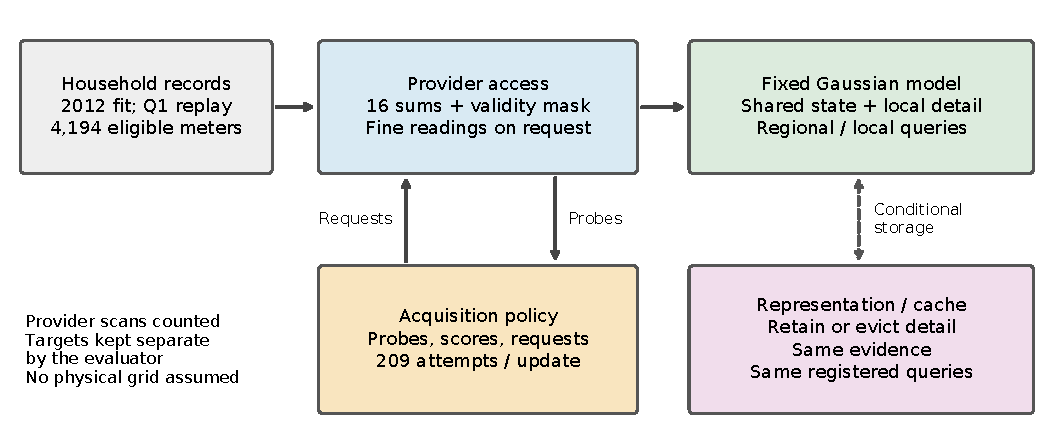
\includegraphics[width=\textwidth]{figures/information_flow.pdf}
\caption{Three distinct operations on one platform. Representation controls retained conditional state. Acquisition controls the household values received. Inference produces regional, group and household queries under one model. All methods receive the same group-summary interface. Reading all meters to construct provider summaries is counted separately from consumer fine access.}
\label{fig:interfaces}
\end{figure*}

\subsection{Provider summaries, fine access and query support}
At each update, the shared provider supplies 16 sums over currently observed households and a native-missingness mask. Thus the actual macro operator includes group totals, not merely one regional total. The evaluator scans the background to construct these summaries; that provider-side scan is charged. Fine readings are available only through a current-cutoff channel that enforces unique requests and a budget. The consumer cannot compute unrevealed household residuals to decide which readings to request.

The restricted methods request at most $\lfloor0.05\times4194\rfloor=209$ household records per update, including 41 rotating probes. Missing requested readings consume an attempt but contribute no likelihood. A 24-step evidence cache stores acquired finite values and expires old entries. Requests, finite returns and assimilation are logged separately. Figure~\ref{fig:interfaces} separates the operations and Table~\ref{tab:methods} defines method interfaces; every method can issue local conditional predictions even when it receives only aggregates.

\begin{table*}[!t]
\caption{Observation and representation interfaces in the shock comparisons. All rows use the same training-fitted model, 16 group sums and missingness masks. Attempts include missing readings. ``Fine'' describes evidence access, not the dimension of the common state.}
\label{tab:methods}\centering
\begin{tabular}{p{.08\textwidth}p{.29\textwidth}p{.28\textwidth}p{.25\textwidth}}
\toprule
Method & Additional current observations & Acquisition rule & Representation and comparison role\\
\midrule
M0 & None & Aggregate change detector & Conditional household predictions remain possible\\
M1 & 41 fixed rotating probes & Same cheap monitoring as M3 & Probe-only information control\\
M2 & 41 probes + 168 random requests & Uniform extra selection, no replacement & Matched 209-attempt simple acquisition\\
M3 & 41 probes + 168 extra requests & Threshold/hold; 42 extra explore, up to 126 target a group & Original event-sensitive refinement\\
M3b & Same 209-attempt budget & Current highest positive score; same exploration & One frozen rank-responsive correction\\
Fixed & Exactly M3 or M3b's sequential trace & Receives no future acquisition decisions & Same-evidence conventional conditional retention\\
M4 & All 4,194 available household readings & Streamed full access & Structured full-information reference\\
\bottomrule
\end{tabular}
\end{table*}

Observed regional targets are sums over the households with a valid target reading. The same support is applied to each method's predictions and uncertainty. This is an evaluator query on the posterior, not a complete-population demand label. Future validity masks enter only these scoring-query weights, not the posterior information matrix or acquisition inputs. Monitoring uses a separate full-support one-step prediction. Neither model selection nor policy sees future consumption. No complete-cohort observed totals were available for the unmodified refinement panel, whose target support ranged from 4,082 to 4,168 households.

\section{What Refinement Can and Cannot Change}
\subsection{Same model, same evidence}
Let $c$ denote retained coordinates and $d$ detail coordinates in a proper Gaussian posterior with precision $J$ and information vector $h$. For $J_{dd}\succ0$, elimination gives
\begin{align}
J_c&=J_{cc}-J_{cd}\operatorname{solve}(J_{dd},J_{dc}),\label{eq:schur}\\
h_c^{\rm marg}&=h_c-J_{cd}\operatorname{solve}(J_{dd},h_d).
\end{align}
The conditional law of $d$ given $c$ has mean $\operatorname{solve}(J_{dd},h_d-J_{dc}c)$ and covariance $J_{dd}^{-1}$. Implementations use factor solves, not explicit matrix inversion. These are standard Gaussian elimination identities underlying distributed and incremental inference~\cite{distributed,isam}.

\begin{proposition}[Registered-query preservation]
Work in exact arithmetic with a fixed model, evidence and window. Suppose a registered query vector has conditional law
$q\mid c\sim\mathcal N(a+Lc,V)$ and $c\sim\mathcal N(m,C)$. Retaining $(a,L,V,m,C)$ preserves its mean $a+Lm$ and covariance $V+LCL^\top$ through eviction of other detail. Exact reconstruction using the corresponding conditionals preserves these quantities and is independent of elimination order.
\end{proposition}
\begin{proof}
The mean follows from iterated expectation. Total covariance gives $V+LCL^\top$. Integrating a proper joint Gaussian over any fixed set of eliminated coordinates gives the same marginal irrespective of integration order. Reconstruction multiplies that marginal by its original conditional law and therefore recovers the same joint distribution.
\end{proof}

The query class matters. The refinement panel registers full-group totals, common observed-support totals and one fixed household per group, separately at each lead. Same-lead cross-covariances are retained. Arbitrary new household combinations or cross-lead joint queries may require reconstruction. A coarse marginal alone is insufficient: $c\sim\mathcal N(0,1)$ is compatible with either $d=c+e$ or $d=-c+e$, for independent $e\sim\mathcal N(0,1)$. The identical coarse law leaves opposite cross-covariances unresolved. Moving conditionals to an uncounted host cache is not a memory reduction.

When new household readings are constituents of an already used group sum, their likelihood cannot be added independently to the old aggregate likelihood. The implemented update uses
\begin{equation}
p(y_{\rm fine},a\mid c)
=p(y_{\rm fine}\mid c)\,p(a\mid y_{\rm fine},c),\label{eq:replace}
\end{equation}
conditioning the derived sum $a$ on acquired values and native masks. Revealing all constituents makes the remaining sum redundant. Evidence versions replace the old group message atomically. A deliberately double-counted update changes the posterior and is retained as a negative control.

With conditionally private groups, a within-window update can reuse unaffected messages but must refactor the common separator. The cost depends on the affected block and its connections, not just the number of new observations. At rank $r=16$, window length $L=24$ and $N$ households, the implementation stores $O(NL^2)$ private temporal covariance plus separator and query summaries; a dense separator factorization costs $O((rL)^3)$. Private temporal factors can be batched on the GPU. Stronger cross-group coupling or fill-in would remove the simple locality. Each moving window here is rebuilt from the fixed training prior. It does not propagate an exact all-history boundary message, and all 16 group factors are rebuilt per sequential shock update.

\subsection{Aggregate visibility}
For household demand perturbation $d_t$ and actual summary operator $S_t$, the observable perturbation is $S_t d_t$. Exact regional cancellation is insufficient if providers also reveal group totals. Our hidden controls cancel within each observed group, including missing-support handling.

For a compatible fixed linear state model, let household demand be $Hx_t$, transition be $F$, and fixed macro mapping be $C=SH$. The standard finite-horizon observability matrix~\cite{hespanha} is
\begin{equation}
\mathcal O_L=\begin{bmatrix}C^\top&(CF)^\top&\cdots&(CF^L)^\top\end{bmatrix}^{\!\top}.
\end{equation}
\begin{proposition}[Finite-horizon indistinguishability]
Compare two linear systems with initial states differing by deterministic $\delta$, identical dynamics and input, and the same joint process and observation noise law. If $\mathcal O_L\delta=0$, their macro observation distributions coincide through time $L$. Any detector based only on those observations, with the same independent randomization, has equal alarm probability under both systems.
\end{proposition}
\begin{proof}
Couple both systems using the same noise draws. Their state difference at time $k$ is $F^k\delta$, so the macro observation difference is $CF^k\delta=0$. Equality almost surely in this coupling implies equality of observation laws, and hence of any measurable detector output law.
\end{proof}

This elementary observability consequence supplies a limit, not a detection algorithm. Additional probe rows can make previously hidden directions visible, but probes that miss the changed households need not do so. Visibility alone supplies no useful finite-sample power guarantee.

For an illustrative pair, changes of $+1$ and $-1$ kWh in one observed group leave its current sum unchanged. If compatible private persistence factors are 0.96 and 0.70, the later sum is $0.96^k-0.70^k$: 0.26 kWh after one step and 0.4316 after two. Equal persistence instead keeps this pair hidden. These numbers illustrate the algebra. The replay disturbances are overlays on measured demand, not draws from this latent-state generator; their visibility is checked directly using $S_t d_t$.

\subsection{From observations to acquisition actions}
The original policy first reads its 41 probes. For acquired meter $i$, it forms $z_{it}=|y_{it}-\widehat y^{\rm coarse}_{it}|/\sqrt{v^{\rm coarse}_{it}}$. The reference is the previous aggregate-only one-step forecast, with a training seasonal initialization. It then updates
\begin{equation}
q_{gt}=0.8q_{g,t-1}+\max\{0,\max_{i\in P_t\cap g}z_{it}-2\},\label{eq:score}
\end{equation}
where an empty probe group contributes zero. If $\max_gq_{gt}>\tau$, with $\tau=13.4334$, M3 selects the highest-scoring group and resets a four-decision hold. Otherwise it retains a held group or becomes inactive. Forty-two of the 168 extra attempts explore; up to 126 target the active group. When inactive, all extra attempts rotate. Probe values can affect the current extra requests. Extra values update inference but never feed the acquisition score, including at the next update.

\begin{proposition}[A sufficient unchanged-gate condition]
Let $b=\max_gq_g$, $b'=\max_gq'_g$, and $e=\|q'-q\|_\infty$. If $e<|b-\tau|$, the strict decisions $b>\tau$ and $b'>\tau$ coincide. The condition does not certify equality when the margin is zero or equality holds.
\end{proposition}
\begin{proof}
The maximum is 1-Lipschitz in the infinity norm, so $|b'-b|\le e$. The stated strict inequality prevents crossing or reaching the threshold from either side.
\end{proof}

An unchanged gate does not alone guarantee unchanged acquisitions. Ranking, ties, hold state, remaining budget and available IDs also matter. We therefore audit actual ordered meter/time requests and finite assimilation, rather than inferring actions from a score or request count. This diagnostic bound is an elementary specialization, not a new event-triggering theorem.

\section{Experimental Protocol}
\subsection{Distinct exploratory cohorts}
We keep three linked but noninterchangeable cohorts. \textbf{A} is unmodified development replay at 32 origins across four weeks, with nested populations of 1,024, 2,048 and 4,194 households. Fixed, random and uncertainty-guided schedules open 2, 4 or 8 groups, producing 864 policy cases and 1,728 restoration cycles. These are computational cases, not independent physical episodes.

\textbf{B} contains 112 sequential episodes on eight backgrounds from the same four development weeks. Six demand-disturbance families, two magnitudes and eight backgrounds give 96 demand episodes; eight unmodified and eight measurement-fault episodes supply controls. Each episode has 23 summary warm-up intervals, 48 scored updates and targets through six hours ahead. Locations, seeds and amplitudes were frozen before comparative scoring.

\textbf{C} is the later corrective check: four predetermined midday backgrounds reused from B, crossed with localized, exactly cancelling, delayed-aggregate and unmodified conditions. It contains 12 fresh-seed demand episodes and four controls. Only the higher nominal magnitude is used. Seed parity makes its localized disturbances increases; it does not cover decreases or all time contexts. Four replayed original episodes support diagnosis but are not pooled into C. The reconstruction of B's 112 episodes likewise adds no independent evidence. Absolute error differences between B and C do not demonstrate temporal model deterioration.

\subsection{Disturbances and targets}
Reversible overlays produce $y^{\rm shock}_t=y^{\rm background}_t+d_t$. Available readings and future demand targets use this same perturbed series. Broad increases are positive controls for macro detection. Localized increases or decreases affect a small subset. Exact opposing changes cancel within a group; approximate cancellation leaves a residual signature. Different positive and negative persistence creates initially hidden changes with later aggregate effects. A ramp tests gradual rather than abrupt local change. A separate sensor-fault control changes readings but leaves targets unchanged.

Magnitudes use training residual scales. Feasible scaling caps decreases at 80\% of available background demand, and paired changes are suppressed on incompatible missing support. Consequently a nominal scale is not always its realized amplitude. We verify cancellation after these operations and preserve null or attenuated realizations rather than selecting easy shocks. There are no invented propagation paths or grid faults. The interventions are synthetic disturbances on real trajectories, not observed physical events or recovered noise-free demand.

\subsection{Calibration, correction and baselines}
The earlier unmodified January 3--4 segment supplies 96 calibration updates. After eight startup updates, empirical quantiles fit acquisition and alarm thresholds. The deployed alarm is an any-channel, per-update maximum over group innovations and legally acquired fine innovations, with a nominal 2\% target. It is distinct from M3's acquisition gate. Each method receives a threshold appropriate to its number and distribution of exposed fine readings. No injected-event labels fit these thresholds.

The one intentional correction, M3b, retains Eq.~\eqref{eq:score}, probes, model, reading budget and exploration. It assigns the already-spent extra budget to the current highest positive score instead of requiring the threshold/hold gate. The alarm remains separately calibrated on the same earlier segment. This was specified before its comparative run; no collection of policy variants was searched. Fixed-representation references receive M3 or M3b's acquired trace sequentially, without future requests, and retain conditionals conventionally. M4 uses structured streamed inference with all currently available readings. The uncertainty-only policy from A is preserved as a diagnostic, not rerun to seek a favorable outcome.

Intervals include future process and measurement uncertainty. Raw central 90\% intervals use 1.6449 standard deviations. Adjusted intervals multiply by empirical absolute standardized-error quantiles from the earlier calibration segment. Serial dependence, model misspecification and adaptive selection prevent interpreting these as exact coverage guarantees. In particular, old acquisition decisions depend on observations no longer present after a window shift; their informative selection effects are not modeled. Same-evidence numerical agreement is therefore equality of the implemented working posterior, not proof that it is the true posterior conditional on every historical action.

\subsection{Metrics and paired evidence}
Detection is any alarm at lags 0 through 6 after onset, inclusive: seven observation instants over three hours. Correct localization requires at least one currently affected group among the alarmed groups in that window. A missed detection is assigned delay seven half-hour steps, so delay averages include failures. We do not convert all event time points into successes after one hit. Negative-control alarms are alarmed updates divided by all unmodified updates; false household and group localizations are retained separately.

Local mean absolute error (MAE) averages valid affected-household errors within a target interval, then intervals during the event, then episodes. B's primary local average uses 80 episodes from the five local families, excluding broad regional shifts and controls. C uses its 12 demand episodes. Forecast phase is based on target time: some event targets were forecast before an unannounced shock was observable. The methods receive no credit for foreknowledge. Regional consequences exclude exactly cancelling events, for which unchanged regional MAE cannot be a refinement benefit.

Comparisons are paired on identical backgrounds, overlays and target support. We show all background-level differences, averaging magnitudes and families within background. Eight backgrounds occupy only four weeks, and C reuses one background per week. We avoid confidence intervals based on independent households or hours, significance claims from the small panel, and interpreting similar averages as equivalence. The frozen alarm operating point is reported with its realized rate; no post hoc score sweep is presented as a closed-loop policy improvement.

\subsection{GPU implementation and resource accounting}
Numerical fitting and replay use FP64 GPU calculations on an NVIDIA RTX PRO 4500 Blackwell with 32,623 MiB reported memory, rather than the unverified 48 GB planning assumption. CPU work handles typed ingestion, provenance, orchestration and saved-output analysis. Inference uses batched household temporal factors and one common separator factor. Means and aggregate covariances are computed by solves, with shared-future-noise terms retained.

Costs distinguish provider scans, consumer requests, serialized payloads, transfers, retained state and complete update latency. Simulated wire bytes are not measured network traffic or Parquet bytes. Ground-truth evaluation does not grant the estimator free fine access. Complete comparison costs include model setup and cache restoration where relevant. We preserve the earlier negative shared-matrix solver result; raw CPU/GPU speedup is not the contribution of this study.

\section{Results}
\subsection{RQ1: preservation without a capacity advantage}
Registered-query means and variances survive representation refinement and eviction in all 864 cases. Policy round trips have zero recorded discrepancy; the broader restoration checks, including streamed fine reconstruction, reach $1.42\times10^{-14}$. Incremental and rebuilt separator means differ by at most $4.14\times10^{-15}$. These FP64 comparisons verify the implementation on tested cases, not a floating-point proof or physical accuracy claim.

At 4,194 households and eight active groups, retained state falls from 61.12 MB to 21.60 MB after eviction. Streamed fine inference also retains 21.60 MB. Thus the apparent saving against a resident implementation does not establish more representable households or an advantage over conventional streaming. Initial summaries, private covariance storage, host caches and later reconstruction remain necessary.

The model supports predictive macro-to-micro and micro-to-macro effects. In a saved first-origin trace, exposing detail alone leaves the regional mean at 988.287 kWh and a selected household mean at 0.5630 kWh. Acquiring eight groups changes these to 984.012 and 0.6666 kWh. An unopened group's selected household changes from 0.5012 to 0.6057 kWh through the common state. These are full-model query means, not complete-population observations or causal demand-response effects. Detail exposure is invariant; new evidence is not.

The uncertainty-guided schedule in the largest cohort remains static because its Gaussian conditional variance score does not depend on newly observed values. With eight groups, one-hour regional MAE is 39.082 kWh versus 37.599 for random selection, a 3.94\% disadvantage. Its nominal 90\% regional interval covers 59.4\% of the 32 scored one-hour origins. This motivates checking observation-sensitive policies but does not establish a defect in a covariance-only rule.

\subsection{RQ2: added information helps prediction, not every detector}
Table~\ref{tab:results} keeps cohorts B and C separate. In B, streamed fine inference reduces local one-hour MAE from M3's 0.1696 to 0.1386 kWh, about 18.3\% relative to M3. M3's difference from random acquisition is much smaller, 0.00145 kWh or 0.85\%. Figure~\ref{fig:paired} shows heterogeneous paired background differences. More fine evidence has value for this local forecast task; the result does not identify an adaptive representation advantage.

Broad magnitude-three increases are detected in all eight backgrounds by every method. This is a case where macro summaries work well. In contrast, all methods, including random and streamed fine, correctly localize zero of B's 16 exact-cancellation events within the detection window. Cancellation hides the perturbation from macro summaries, but revealing fine values is not sufficient for the deployed detector to cross its threshold. The full-information forecast benefit must not be relabeled a localization success.

\begin{table*}[!t]
\caption{Principal exploratory results, generated from per-episode artifacts. Local one-hour MAE is in kWh per affected household and uses 80 local episodes in B, 12 in C. Detection and correct-group localization use all 96 and 12 demand episodes respectively. Negative alarms use only unmodified controls. Delay includes misses at 3.5 h. Fixed same-evidence representations equal their source policy and are omitted as duplicate rows.}
\label{tab:results}\centering
\begin{tabular}{lrrrrr}\toprule
Method & Local MAE & Detected & Localized & Alarmed control updates & Mean delay (h)\\\midrule
\multicolumn{6}{l}{\textit{Cohort B}} \\
M0 & 0.1777 & 37/96 & 20/96 & 36/384 & 2.44 \\
M1 & 0.1762 & 17/96 & 11/96 & 15/384 & 3.03 \\
M2 & 0.1710 & 33/96 & 14/96 & 25/384 & 2.64 \\
M3 & 0.1696 & 29/96 & 15/96 & 30/384 & 2.66 \\
M4 & 0.1386 & 42/96 & 15/96 & 41/384 & 2.24 \\
\multicolumn{6}{l}{\textit{Cohort C}} \\
M0 & 0.2752 & 10/12 & 5/12 & 19/192 & 1.38 \\
M2 & 0.2667 & 8/12 & 2/12 & 14/192 & 2.17 \\
M3 & 0.2621 & 6/12 & 2/12 & 15/192 & 2.29 \\
M3b & 0.2660 & 4/12 & 2/12 & 14/192 & 2.71 \\
M4 & 0.2053 & 9/12 & 3/12 & 31/192 & 1.33 \\
\bottomrule\end{tabular}

\end{table*}

\begin{figure*}[!t]
\centering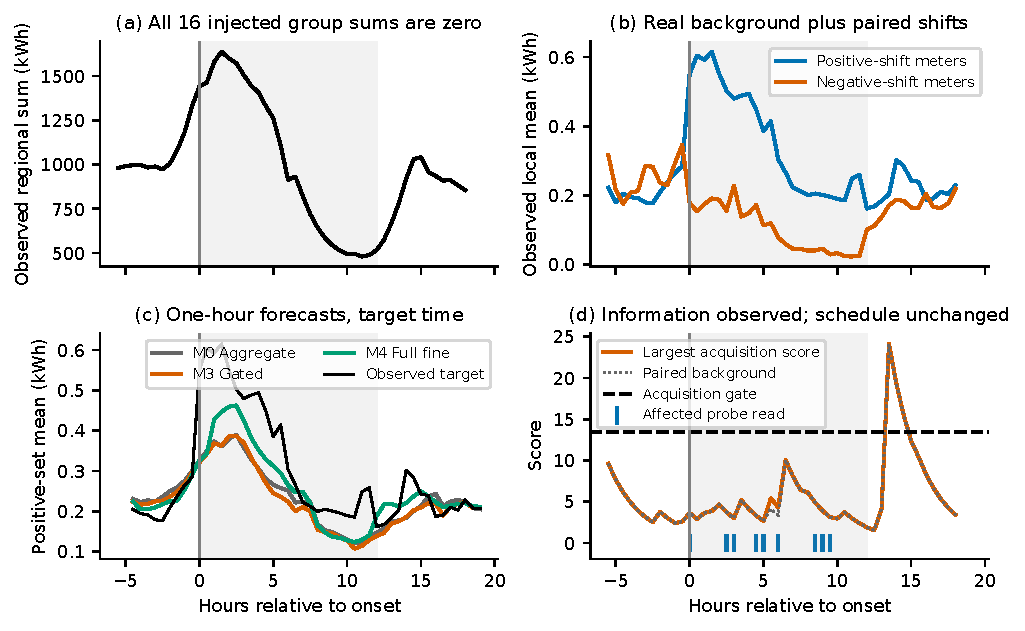
\includegraphics[width=\textwidth]{figures/transparent_episode.pdf}
\caption{Preselected example b00, exact cancellation, nominal magnitude three, chosen by first background and fixed family/magnitude before method comparison. Gray shading marks the disturbance. (a) The observed-support regional total varies with real background demand, but the injected signature is zero in every group. (b) Positive and negative meter sets change locally. (c) One-hour forecasts are aligned to target time and common observed support; they need not anticipate onset. (d) Affected probes change scores during the event without crossing the gate. The later trigger also occurs on the paired unmodified background. Unchanged acquisition and missed localization are retained. Local sets are evaluator labels, never policy inputs.}
\label{fig:episode}
\end{figure*}

Figure~\ref{fig:episode} provides an observed-but-not-acted-on example, selected by a fixed rule. The affected group is 4, with 60 actually affected households. Affected probes appear at onset and on nine event updates. Their normalized innovation reaches 3.4411, while the maximum acquisition score remains at most 10.0537, below 13.4334. The regional injection remains zero. The example illustrates information reaching the consumer without useful acquisition or localization, rather than selecting a successful anecdote.

The streamed reference costs more information. Across B, M3 requests 1,123,584 fine records, receiving 1,106,434 finite readings, whereas M4 requests 22,546,944 and receives 22,204,000. Fine-plus-summary payload estimates are approximately 22.52 MB and 364.95 MB, a 16.2-fold difference at the consumer interface. The shared provider still scans all 4,194 meters to form each summary. Dense masked arrays produce about 5.50 GB of host-to-device input transfers per method over the comparison, so the wire saving is not a measured transfer or provider-computation saving.

Retained separator state after detail eviction is approximately 2.365 MB per shock update for M3 and M4. The fixed-retention comparator temporarily retains approximately 41.017 MB; shared private covariance accounts for a further 38.652 MB and a host evidence cache about 0.805 MB per method. Peak GPU allocation for the comparison is about 182.49 MB, with 1.73 GB peak host memory. All 16 group messages are rebuilt per moving-window update. Complete updates are around 72 ms at the median, with similar values across these methods. These costs reveal no new locality or capacity gain over the streamed comparator.

\begin{figure*}[!t]
\centering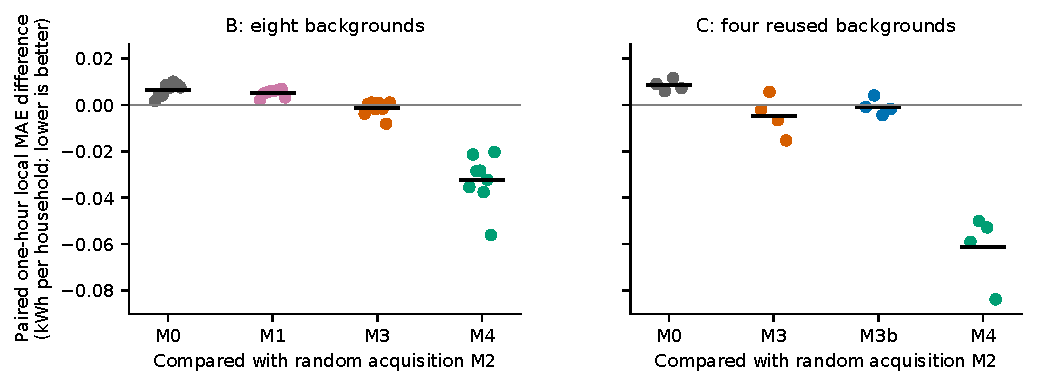
\includegraphics[width=\textwidth]{figures/paired_comparison.pdf}
\caption{Paired local one-hour MAE differences from random acquisition M2. Each dot is a background average, with magnitudes/families averaged inside that background; black bars show the mean. Lower is better. B has eight backgrounds in four weeks; C uses four of those backgrounds with fresh seeds and different conditions. They are separate panels, not successive estimates of one population error. The displayed spread is descriptive, not an independent-household confidence interval.}
\label{fig:paired}
\end{figure*}

\subsection{RQ3: information reaches scores but not useful actions}
The reconstruction reproduces all 5,376 original ordered request traces, finite return counts and active-group states. Identity hashes include actual meter IDs and timestamps; maximum score reconstruction discrepancy is $1.60\times10^{-14}$. All 96 demand episodes expose an affected fine reading, and 94 expose an affected probe. Innovations differ in 96 cases, group scores in 93, full rankings during the event in 86, and the top-ranked group in 17. Nevertheless, no trigger, active action or actual acquisition schedule changes. There are no budget rejections. Controlled large-innovation tests through the same path do change actions when an alternative is available, excluding an inherently disconnected scheduler.

The diagnostic condition strengthens this account. At all \MarginChecks{} paired demand-episode updates, the maximum score-vector perturbation is strictly smaller than the paired background's distance to the acquisition gate (Fig.~\ref{fig:path}). Thus none can switch the threshold bit by Proposition 3. Unchanged final actions are established separately by the trace comparison, since a stable gate would not by itself exclude rank or hold effects. Three cases lose their changes at the group maximum/drift step. Two lack a direct probe hit but change the probe reference through macro observations. No lost shock overlay, indexing defect or later scheduler overwrite was found.

The original alarm rate is 30/384 unmodified updates, or 7.81\%, against the nominal 2\% calibration target. Both are any-channel/update quantities, not a per-household versus family-wise mismatch. Matching the calibration's eight-update startup exclusion still gives 17/320, or 5.31\%, versus 2/88 calibration updates. Startup explains part, not all, of the discrepancy. Unmodified backgrounds can contain genuine unlabeled anomalies; these are false alarms relative to the injected-event protocol, not verified false physical incidents.

M3b changes schedules in three of C's 12 demand episodes. It, M3 and random acquisition each correctly localize two. Its local MAE is 0.2660 kWh versus 0.2621 for M3, 0.2667 for random and 0.2053 for streamed fine. The 0.25\% average reduction from random is inconsistent across backgrounds and does not establish a policy benefit. The original M3 is better on the primary average. M3b's negative-control rate is 14/192, or 7.29\%, compared with M3's 15/192, or 7.81\%; neither meets the intended rate. Limited-access methods retain 209 attempts per update and the same 2.666 MB fine-payload estimate across C, with small differences in finite returns.

\begin{figure*}[!t]
\centering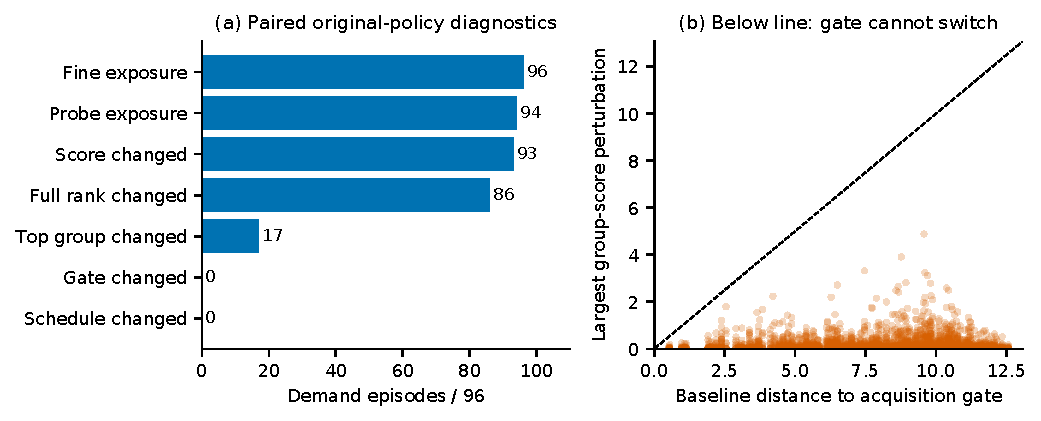
\includegraphics[width=\textwidth]{figures/acquisition_path.pdf}
\caption{Observation-to-action diagnosis in B. (a) Counts use 96 demand episodes; rank changes are evaluated during the disturbance, while changed-score checks cover the replay. These are distinct conditions, not independent successes in a strict funnel. (b) Each nonzero paired score perturbation is compared with the baseline gate margin. All 4,608 update comparisons satisfy the strict sufficient unchanged-gate condition, including zero perturbations omitted from the scatter. Final schedule identity is verified from meter/time traces, not inferred from this bound alone.}
\label{fig:path}
\end{figure*}

The saved corrective traces explain part of this failure. In the changed exact-cancellation episode, new selection first appears at lag eight, outside the lag-0-through-6 detection window. One localized episode first changes at lag nine. These changes add 120 and 77 requests for event-affected meter IDs during the later event, respectively. The remaining localized episode changes once at lag six but adds no affected meter ID. Thus no changed request adds an event-affected identity inside the scored detection window. Counts by identity alone do not establish a finite nonzero reading at every such instant; the separate opportunity audit uses actual masks and perturbations.

Moreover, in every fresh demand episode the largest acquired fine innovation within that window is at most 15.85, below M3b's effective fine alarm threshold of 20.586. Its two correct-group localizations therefore arise through the macro alarm channel, not a newly triggered household alarm. M3b's calibration raises that effective threshold from M3's 19.708. These observations explain why responsiveness did not improve the recorded localization result. They do not prove that faster targeting or another threshold would work: changed acquisitions alter later evidence, and fixed-trace rescoring cannot evaluate that closed loop.

Under identical evidence, fixed and adaptive representations agree in all 5,376 original comparisons and 960 corrective/diagnostic updates. Conditional retention is therefore not the source of the forecast differences. The benefit demonstrated here is predominantly the extra evidence available to streamed fine inference, not a new representation or a reliably superior acquisition policy.

\section{Discussion and Limitations}
For data-space consumers, an interface should specify which summaries are derived from which records, which current fine readings may be requested, and which query laws survive eviction. A change in display or retained state need not change information. Conversely, a low-rank model can already consume every household reading. These distinctions prevent an apparent macro-to-micro improvement from being attributed to the wrong mechanism.

The empirical diagnostic also separates allocation from alarming. The original gate was calibrated as a high quantile of background scores, then used to decide where to spend a budget that would be spent regardless. Informative ranking changes remained below that gate. Removing it made some decisions responsive, but the altered reads were too late for the scored window and fine alarm thresholds still rejected every fresh demand case. The measured failure is therefore more specific than ``the policy did not adapt.'' It identifies a decision margin, an acquisition timing mismatch and a remaining detection limitation.

Uncertainty quality remains inadequate. The earlier 59.4\% regional coverage is not explained by a missing future-noise term: code and independent covariance checks include process noise, measurement noise and aggregation covariance. In B's unmodified controls, M3's raw one-hour regional coverage is 72.14\% with mean width 106.01 kWh. Empirical adjustment widens it to 149.31 kWh and raises coverage to 84.12\%, still below 90\%. Wider intervals do not validate the model or repair acquisition. Adaptive selection outside the retained window, nonstationary demand, common-model errors and the chosen private-noise convention all limit interpretation.

The study has only four development weeks. Repeated investigation and one correction use development findings, and fresh synthetic seeds on reused backgrounds are not held-out real-world validation. Injection families, amplitudes and onset contexts do not represent an estimated distribution of actual disruptions. The regional twin covers a sampled household population without physical grid topology. Missing-support totals cannot establish complete-population performance. The negative alarm controls may contain unlabeled real changes, and the simple detectors are not a state-of-the-art anomaly benchmark.

Resource claims are similarly bounded. The archive is substantial, but the 384-dimensional common separator is small. Structured streaming already fits easily on the measured GPU. Retained-state accounting excludes some shared arrays by definition, so total peaks and cache costs are reported separately. The implementation's dense masked transfers and full group reconstruction at every window shift leave substantial engineering limitations. No GPU-versus-CPU superiority, production throughput, distributed availability, privacy or physical resilience follows from this single-machine replay.

One precise next question remains: under a fixed number of legally acquired probes, can earlier observation-driven group ranking deliver additional affected readings before a predeclared detection deadline, while controlling the deployed alarm rate on separate chronological backgrounds? This requires a new frozen study, not a threshold sweep on the present traces. The current evidence supplies a failure diagnosis and experimental controls for that question, not its answer.

\section{Conclusion}
More detail has three meanings in a regional twin: exposing conditional state, acquiring additional observations, and choosing those observations. On this London prototype, same-evidence representation changes preserve registered queries but establish no capacity advantage over streamed fine inference. Additional fine readings improve local forecasting under synthetic disturbances, while aggregate blindness and a conservative fine detector still prevent successful localization of exactly cancelling events. The original acquisition gate blocks measured score changes; a single rank-responsive correction changes a few schedules without a demonstrated detection or prediction advantage. Auditing the full observation-to-action path, with matched evidence and explicit resource accounting, is the supported contribution of this exploratory case study.

\bibliographystyle{IEEEtran}
\bibliography{references}
\end{document}
